
\documentclass[12pt,a4paper]{report}
\usepackage{graphicx}
\usepackage[utf8]{inputenc}
\DeclareUnicodeCharacter{00A0}{\nobreakspace}
\usepackage[T1]{fontenc}
\usepackage[english]{babel}
\usepackage{times}
\begin{document}
\begin{titlepage}
\thispagestyle{empty}

\vspace{0.2in}

\begin{center}
{\Huge{}expEYES-17}
\par\end{center}{\Huge \par}

\begin{center}
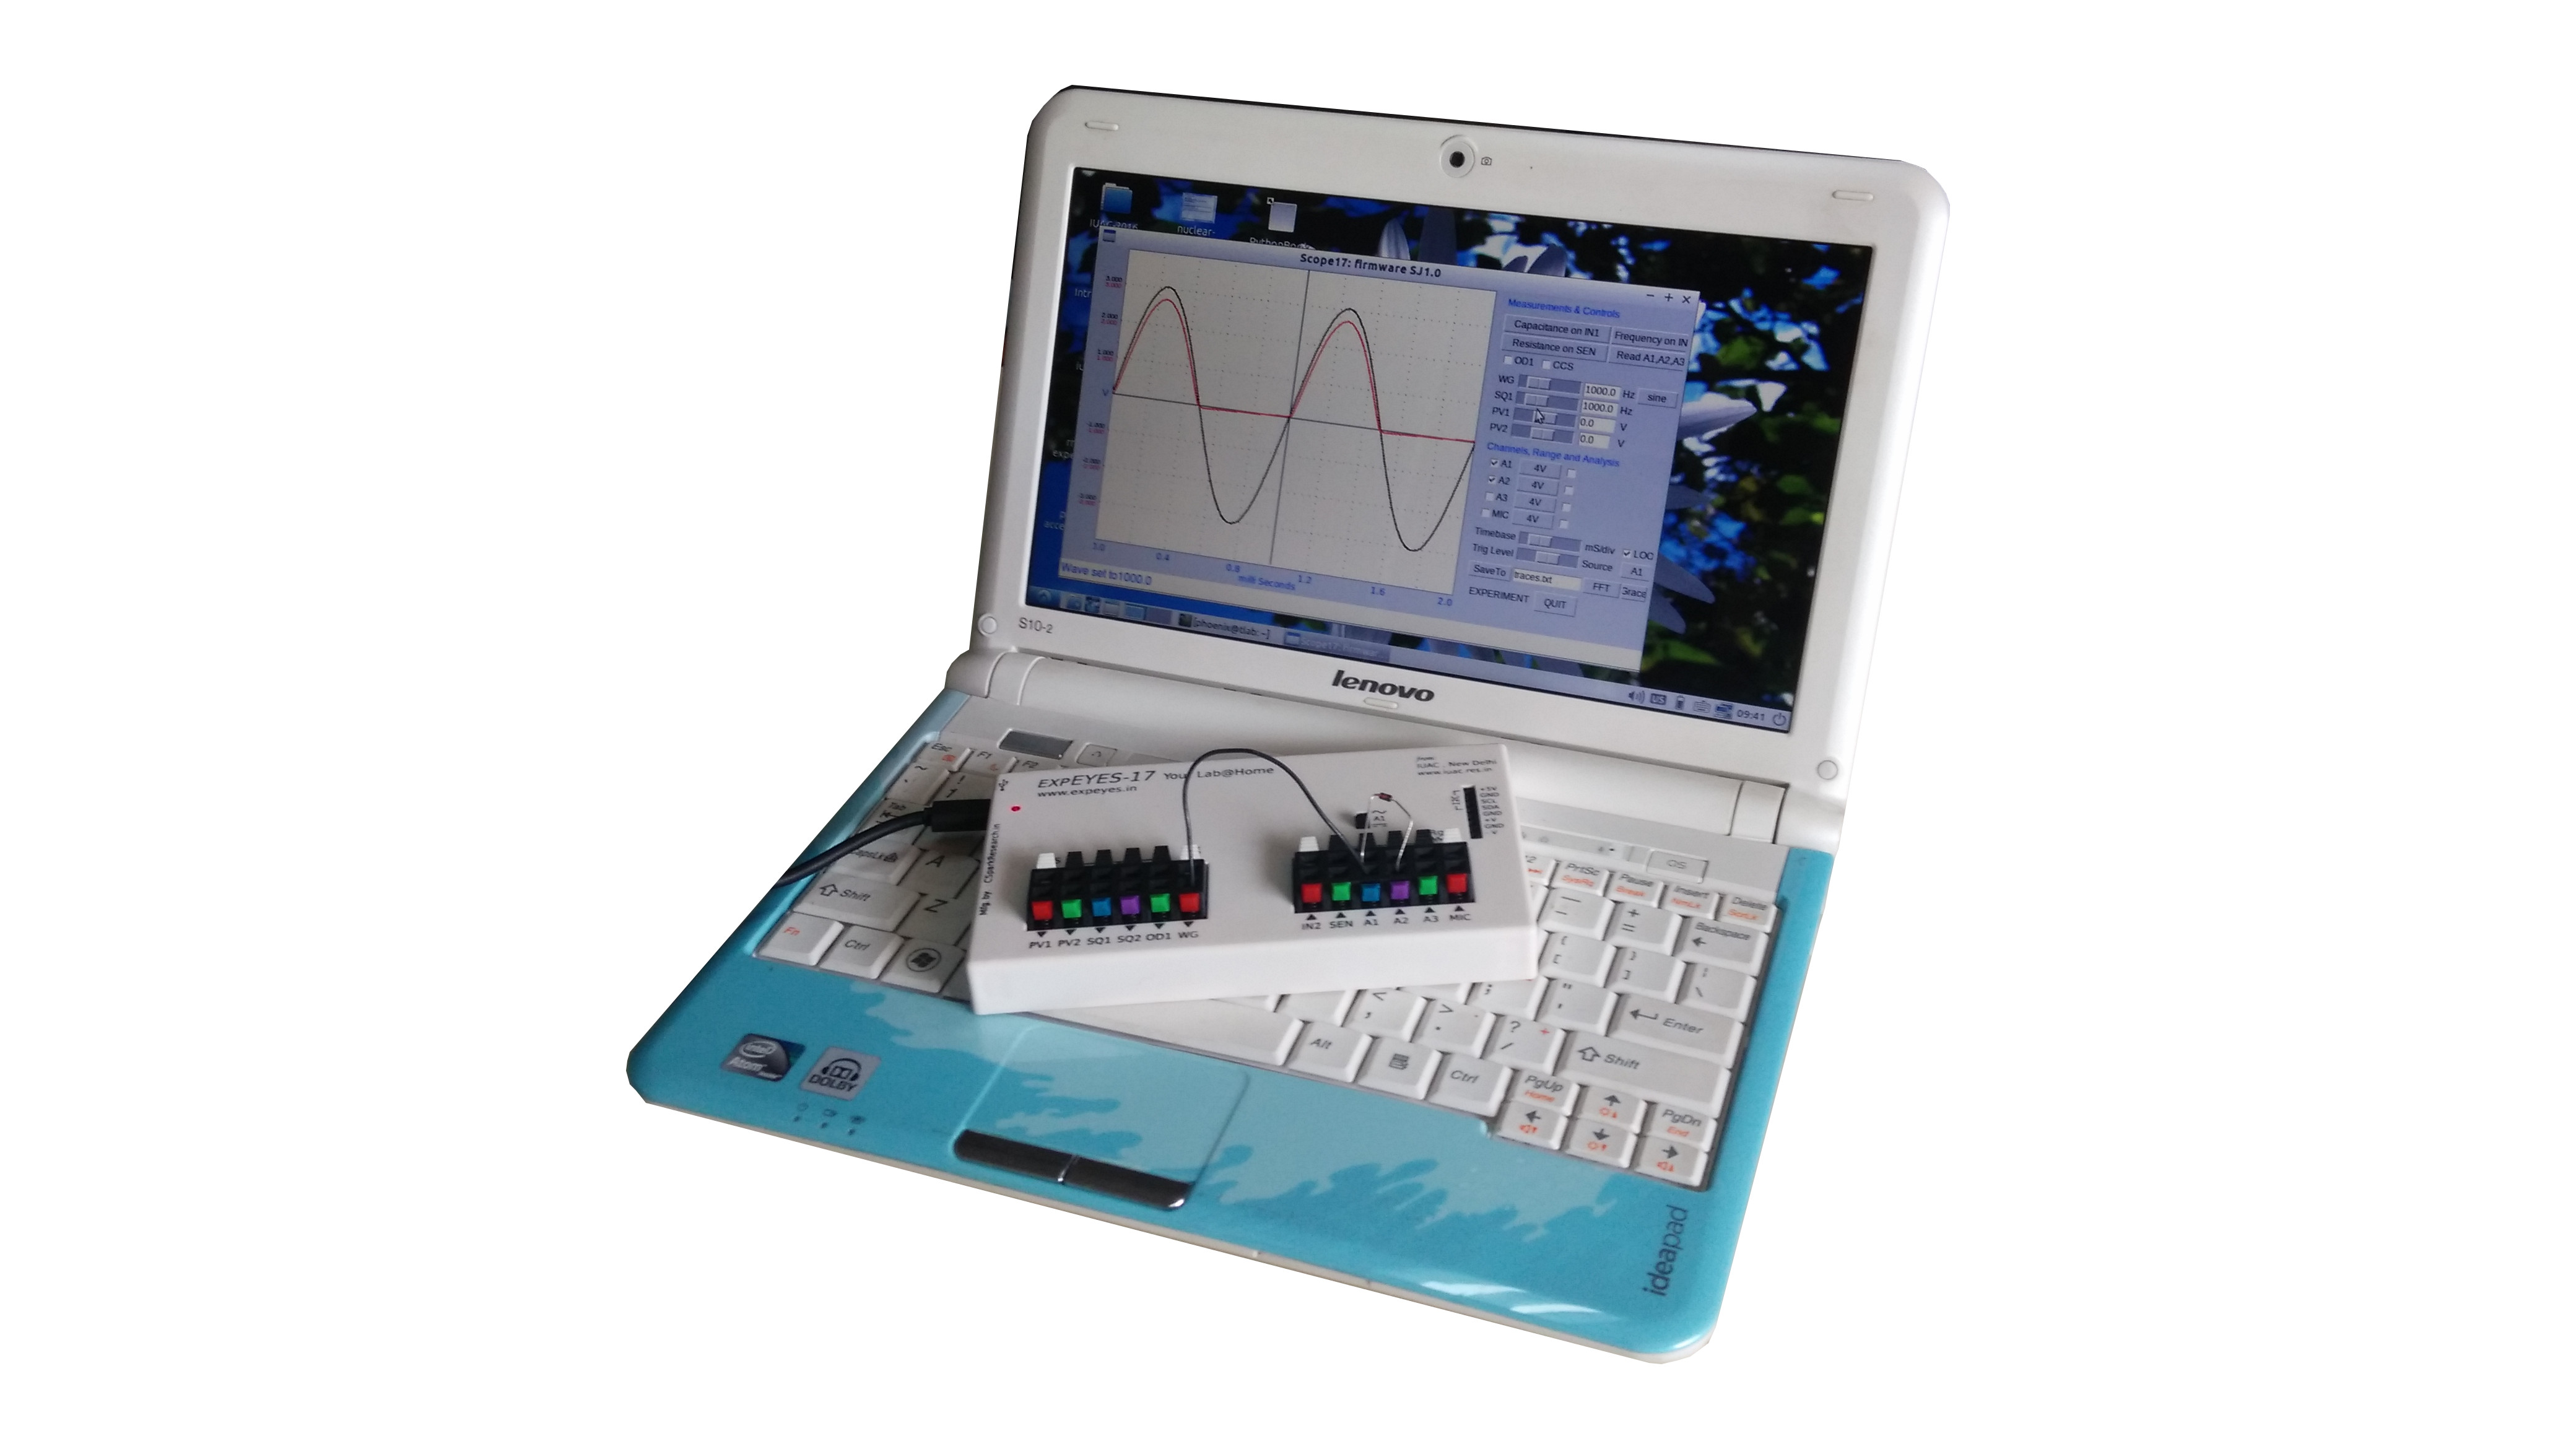
\includegraphics[width=6cm]{../../pics/eyes17-nb}
\par\end{center}

\begin{center}
{\large{}സഹായഗ്രന്ഥം  }
\par\end{center}{\large \par}

\begin{center}
{\LARGE{} യുവശാസ്ത്രജ്ഞർക്കും സാങ്കേതികവിദഗ്ദ്ധർക്കുമുള്ള}\\
{\LARGE{}  പരീക്ഷണങ്ങൾ }
\par\end{center}{\LARGE \par}

\begin{center}
http://expeyes.in
\par\end{center}

\begin{center}
from
\par\end{center}

\begin{center}
PHOENIXപ്രൊജക്റ്റ് \\
ഇന്റർ യൂണിവേഴ്സിറ്റി ആക്സിലറേറ്റർ സെന്റർ  \\
(UGCയുടെ ഒരു ഗവേഷണസ്ഥാപനം )\\
ന്യൂ ഡൽഹി  110 067\\
www.iuac.res.in
\par\end{center}

\end{titlepage}
\end{document}

